\begin{figure}[!htbp]
    \centering
    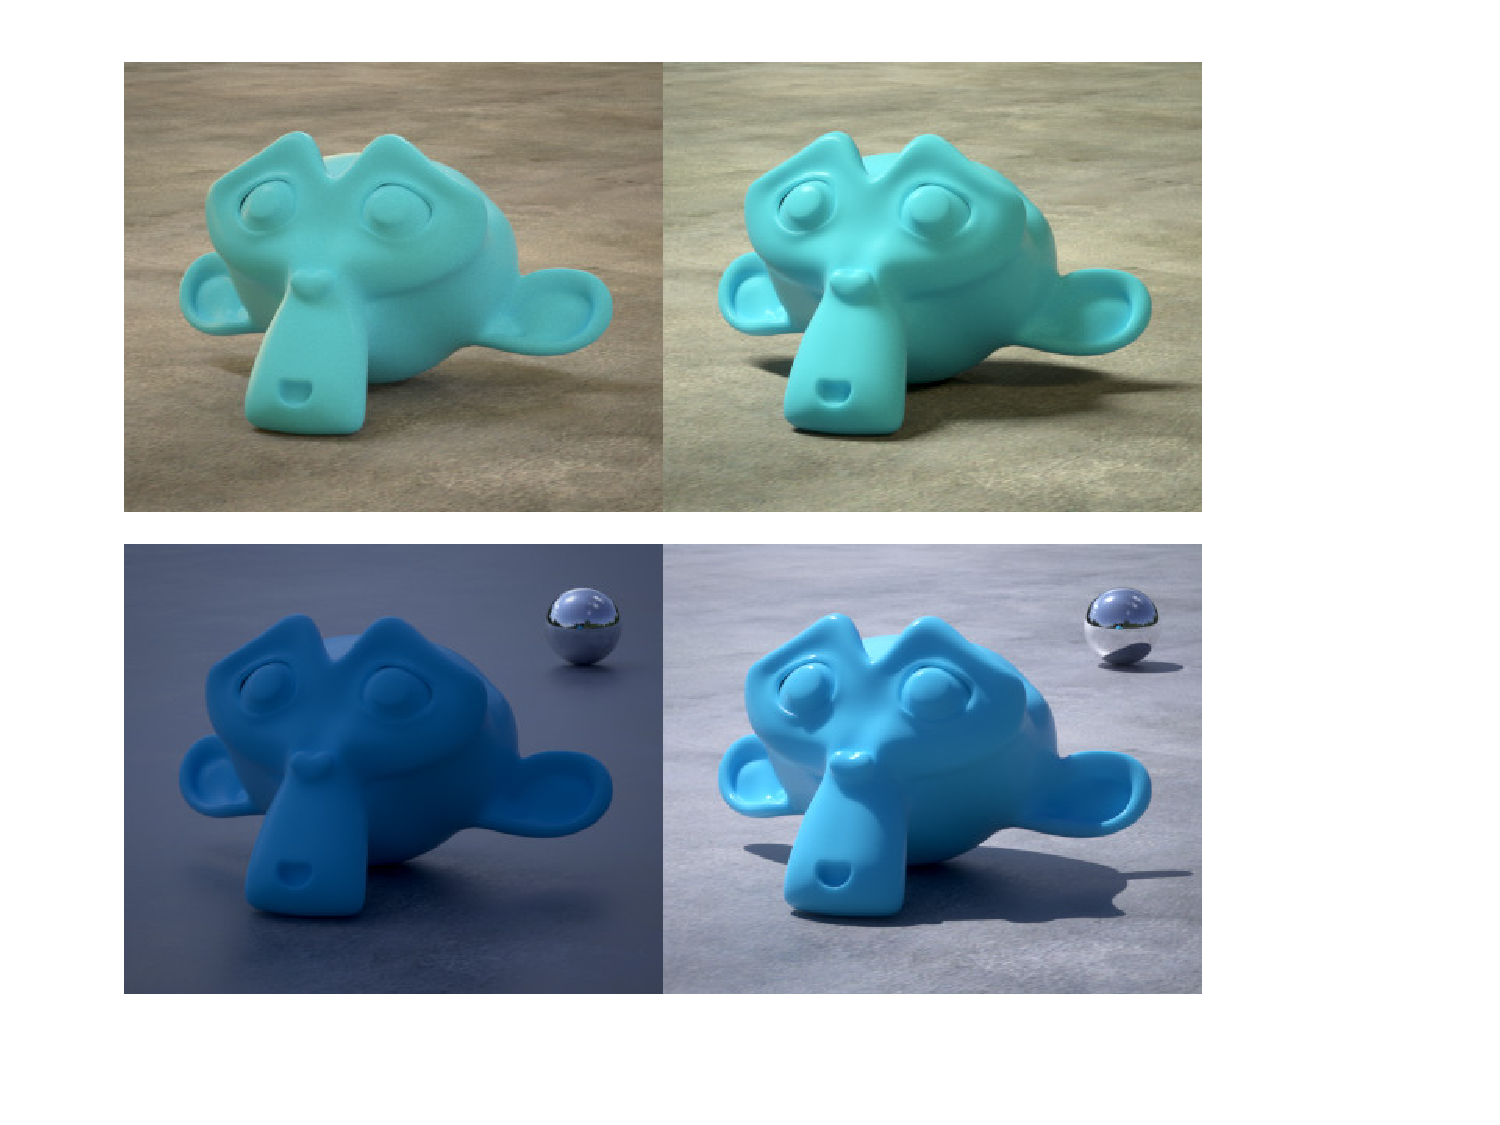
\includegraphics[width=1.0\textwidth]{Img/hdr-render.pdf}
    \caption[使用HDR全景图与LDR全景图渲染结果的对比]
    {使用LDR全景图(左)与使用HDR全景图(右)渲染结果的对比,引自\cite{makehdr}。从第一行可以看出,使用低动态范围全景图像渲染的结果,在颜色上对比平缓,看起来很不真实。而使用HDR全景图渲染的结果提供了足够的对比度和锐利的阴影,更具有真实感。这种情况在场景中有较强光线时尤为明显(第二行结果)}
    \label{fig:hdr-render}
\end{figure}